\subsubsection{Numerical verification at small intervals}
\label{sec:num-boson-small}
The current contribution predicts $\alpha=2$ in all six directions.
The leading amplitudes for $00\leftrightarrow ss$,
$00\leftrightarrow3s,s$, and $ss\leftrightarrow3s,s$ are
$\pi^2/12$, $5\pi^2/12$, and $\pi^2/6$, respectively.
Figure~\ref{fig:num-boson-small} compares these predictions with the
reduced-state calculation, and Table~\ref{tab:num-boson-small}
separates the free-power estimates from the fixed-power amplitudes.
The free exponents range from $1.9649$ to $1.9983$, supporting the
quadratic leading behavior. The two-term fits use powers two and
four and bring every leading amplitude closer to CFT than $F_1$.
Their remaining discrepancies are approximately $-5.17\%$ for
$00\leftrightarrow ss$, $-3.60\%$ for $00\leftrightarrow3s,s$, and
$-1.05\%$ for $ss\leftrightarrow3s,s$.

These amplitude offsets are visible in
Fig.~\ref{fig:num-boson-small-residual}. Increasing $N$ makes $x$
small while keeping the subsystem resolution fixed at six to ten
sites; it does not by itself establish a continuum extrapolation.
Omitting each chain size in turn, $F_2$ improves prediction over
$F_1$ in four of the six directions. For $00\mid ss$ and
$ss\mid00$, the prediction error instead increases by about
$2.57\%$ and $2.58\%$. The fitted fourth-order amplitudes therefore
describe corrections over this window; they are not independently
verified analytical coefficients.
% Condensed from numerical/tables/boson_small_parameters.tex; numerical values copied without refitting.
\begin{table}[htbp]\centering\footnotesize
\setlength{\tabcolsep}{3.5pt}
\begin{tabular}{lrrrrrrr}\toprule
Direction & $\widehat\alpha$ & $C_{\rm free}$ & $c_0^{\rm CFT}$ & $c_0(F_1)$ & $c_0(F_2)$ & $c_1(F_2)$ & $\eta_0(F_2)$\\\midrule
$00\mid ss$ & 1.9982 & 0.77501 & 0.82247 & 0.77866 & 0.77996 & -0.1917 & -5.1687\\
$ss\mid 00$ & 1.9983 & 0.77529 & 0.82247 & 0.77871 & 0.77995 & -0.18219 & -5.1696\\
$00\mid 3s,s$ & 1.9649 & 3.5315 & 4.1123 & 3.8623 & 3.964 & -15.02 & -3.6065\\
$3s,s\mid 00$ & 1.966 & 3.545 & 4.1123 & 3.8657 & 3.9643 & -14.541 & -3.6009\\
$ss\mid 3s,s$ & 1.9883 & 1.5661 & 1.6449 & 1.6134 & 1.6276 & -2.0896 & -1.0534\\
$3s,s\mid ss$ & 1.9902 & 1.576 & 1.6449 & 1.6157 & 1.6276 & -1.7507 & -1.0534\\
\bottomrule\end{tabular}
\caption{Compact-boson small-interval fits on $0<x\leq0.1$, with 598 geometries per direction. The free fit is $C_{\rm free}x^{\widehat\alpha}$; $F_1,F_2$ impose the powers in Table~\ref{tab:num-powers}. All amplitudes include powers of $\pi$. The final column is the signed leading-amplitude discrepancy of $F_2$ in percent, Eq.~\eqref{eq:num-residuals}. The $c_1$ column gives a fitted next amplitude, not a theoretical prediction.}
\label{tab:num-boson-small}
\end{table}

\begin{figure}[p]\centering
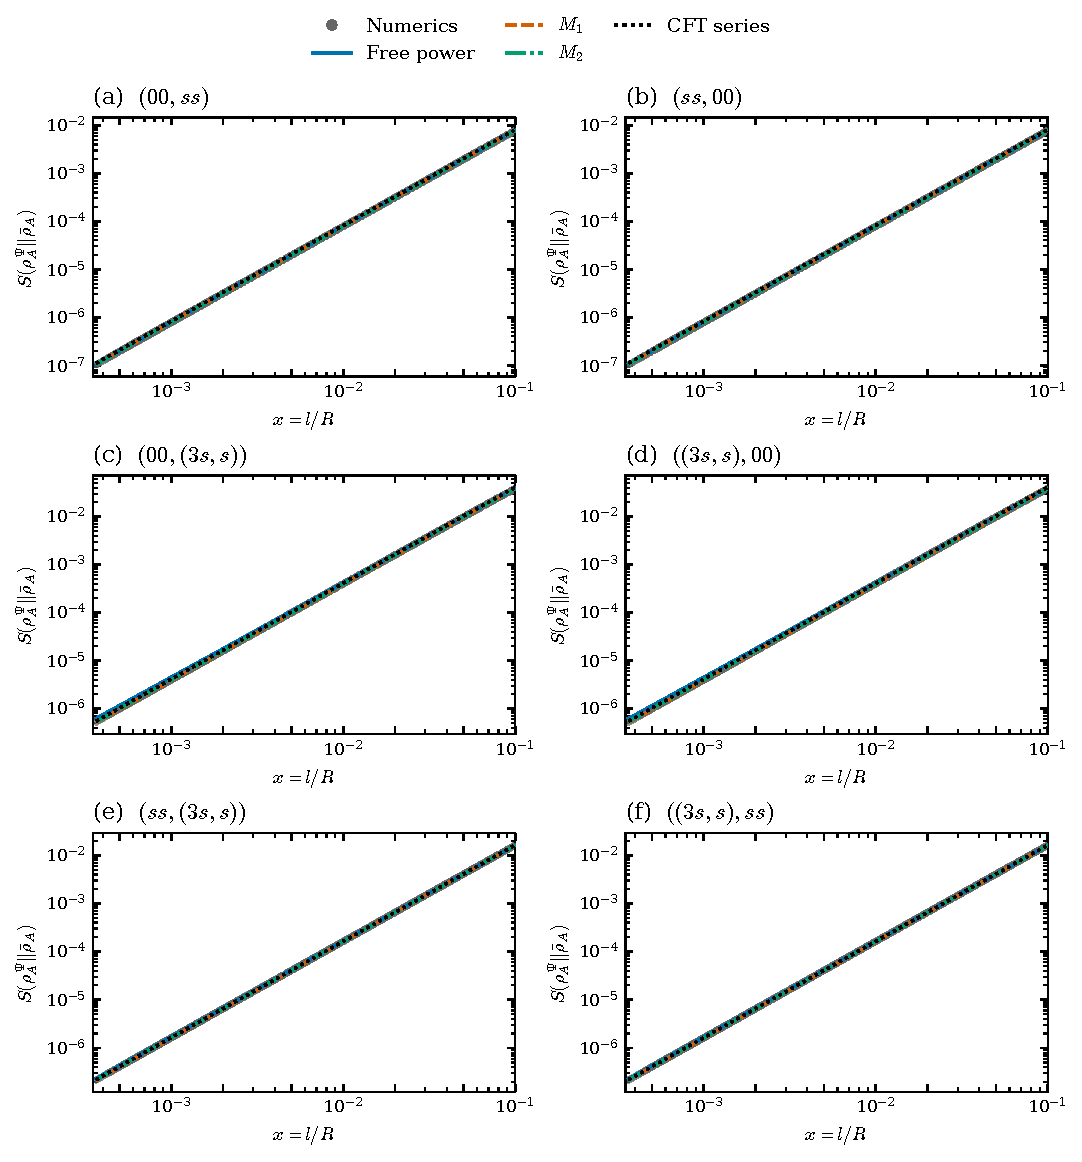
\includegraphics[width=.94\linewidth,height=.74\textheight,keepaspectratio]{figs/boson_small_fit_window_value.pdf}
\caption{Compact-boson small-interval $D^A_{a\mid b}$ for all six ordered pairs. All 598 displayed geometries per direction lie in the fitting window $0<x\leq0.1$, with $\ell=6,\ldots,10$. Both axes are logarithmic. Gray circles denote numerical data, using the same shape and color for every subsystem length. Blue solid, orange dashed, and green dash--dotted curves denote the free fit, $F_1$, and $F_2$; black dotted denotes the parameter-free CFT series. All curves are restricted to the fitting window.}
\label{fig:num-boson-small}
\end{figure}

\begin{figure}[p]\centering
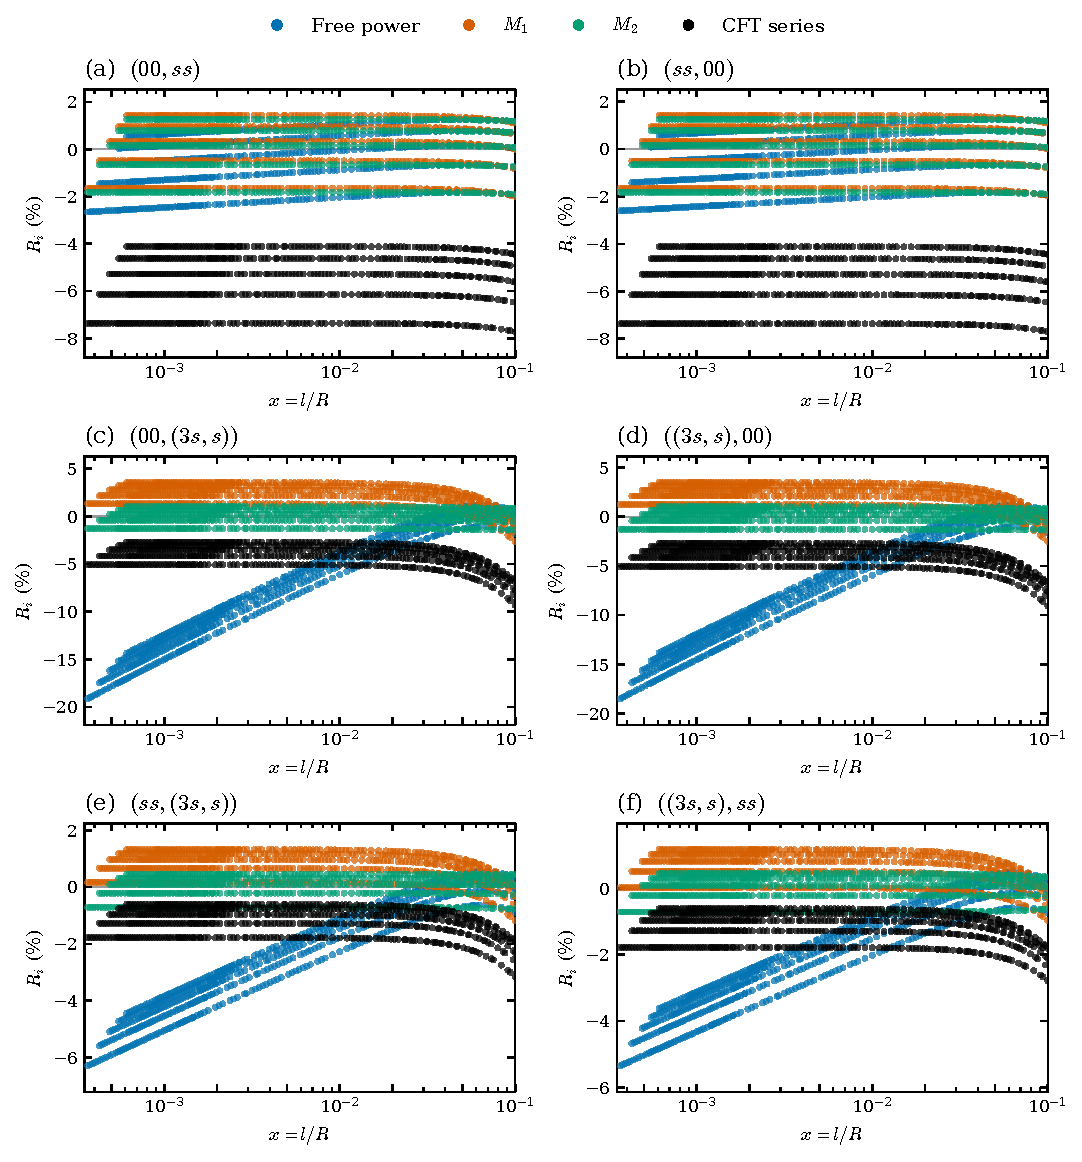
\includegraphics[width=.94\linewidth,height=.74\textheight,keepaspectratio]{figs/boson_small_fit_window_residual.pdf}
\caption{Signed percentage residuals $100[q-M]/q$ for Fig.~\ref{fig:num-boson-small}, with $q=D^A$. The residual ordinate is linear and the fraction axis logarithmic. Only the 598 fitted geometries per direction at $0<x\leq0.1$ are shown. All subsystem lengths $\ell=6,\ldots,10$ use circular markers; colors identify models and are identical across lengths. Blue, orange, green, and black denote the free fit, $F_1$, $F_2$, and the parameter-free CFT series.}
\label{fig:num-boson-small-residual}
\end{figure}

\clearpage

\subsubsection{Numerical verification at large intervals}
\label{sec:num-boson-large}
The deficit resolves the approach to $D^B_{a\mid b}=\log2$.
For the same three unordered pairs, theory predicts
\begin{equation}
 (\beta,c_0^{\rm CFT})=
 (1,\pi^2/8),\quad (5,5\pi^6/64),\quad (2,\pi^2/3),
 \label{eq:num-boson-large-leading}
\end{equation}
with the same leading term in both directions.
Figure~\ref{fig:num-boson-large} and
Table~\ref{tab:num-boson-large} show free exponents within
$0.44\%$ of these predictions. In particular, the fifth-power
channel gives $\widehat\beta=4.9836,4.9838$. Its two-term leading
amplitudes, $74.307,74.252$, differ from $5\pi^6/64\simeq75.109$
by $-1.07\%,-1.14\%$, respectively.

At the adopted cutoff $\ep=0.005$, $F_2$ improves the leading
amplitude in four of six directions and improves omitted-size
prediction in only two. The exceptions to amplitude improvement
are $00\leftrightarrow ss$: the $F_1$ error of about $+2.26\%$
becomes about $+2.35\%$ with $F_2$. Prediction improves only for
$ss\leftrightarrow3s,s$; even the fifth-power pair has a small
negative prediction gain. Figure~\ref{fig:num-boson-large-residual}
shows the residuals against both fitted and analytical curves.
The second term for $ss\leftrightarrow3s,s$ tests the allowed
$\ep^3$ sector, whose complete coefficient has not been established
analytically. Its fitted value must not be taken as proof that this
sector survives the full replica continuation.

The amplitude comparison is sensitive to the upper endpoint.
The supplied cutoff scan finds an all-six amplitude improvement
only for the single data selection represented by
$0.0046916890\leq\ep_{\max}<0.0047418335$; the weakest gain there
is about $0.00555$ percentage points. No admissible scanned window
improves both amplitude accuracy and omitted-size prediction in
all six directions. We therefore report the prescribed $0.005$
window and its exceptions explicitly.
% Condensed from numerical/tables/boson_large_parameters.tex; numerical values copied without refitting.
\begin{table}[htbp]\centering\footnotesize
\setlength{\tabcolsep}{3.5pt}
\begin{tabular}{lrrrrrrr}\toprule
Direction & $\widehat\beta$ & $C_{\rm free}$ & $c_0^{\rm CFT}$ & $c_0(F_1)$ & $c_0(F_2)$ & $c_1(F_2)$ & $\eta_0(F_2)$\\\midrule
$00\mid ss$ & 0.99926 & 1.2561 & 1.2337 & 1.2616 & 1.2627 & -0.33376 & 2.3499\\
$ss\mid 00$ & 0.99924 & 1.256 & 1.2337 & 1.2616 & 1.2627 & -0.34138 & 2.351\\
$00\mid 3s,s$ & 4.9836 & 66.924 & 75.109 & 73.093 & 74.307 & -265.58 & -1.0676\\
$3s,s\mid 00$ & 4.9838 & 66.96 & 75.109 & 73.058 & 74.252 & -261.18 & -1.141\\
$ss\mid 3s,s$ & 1.9914 & 3.069 & 3.2899 & 3.2185 & 3.2529 & -8.6617 & -1.1234\\
$3s,s\mid ss$ & 1.9912 & 3.0643 & 3.2899 & 3.2176 & 3.2528 & -8.8758 & -1.1274\\
\bottomrule\end{tabular}
\caption{Compact-boson large-interval fits on $0<\ep\leq0.005$, with 317 geometries per direction. The free fit is $C_{\rm free}\ep^{\widehat\beta}$; $F_1,F_2$ impose the powers in Table~\ref{tab:num-powers}. All amplitudes include powers of $\pi$. The final column is the signed leading-amplitude discrepancy of $F_2$ in percent, Eq.~\eqref{eq:num-residuals}. The $c_1$ column gives a fitted next amplitude, not a theoretical prediction.}
\label{tab:num-boson-large}
\end{table}

\begin{figure}[p]\centering
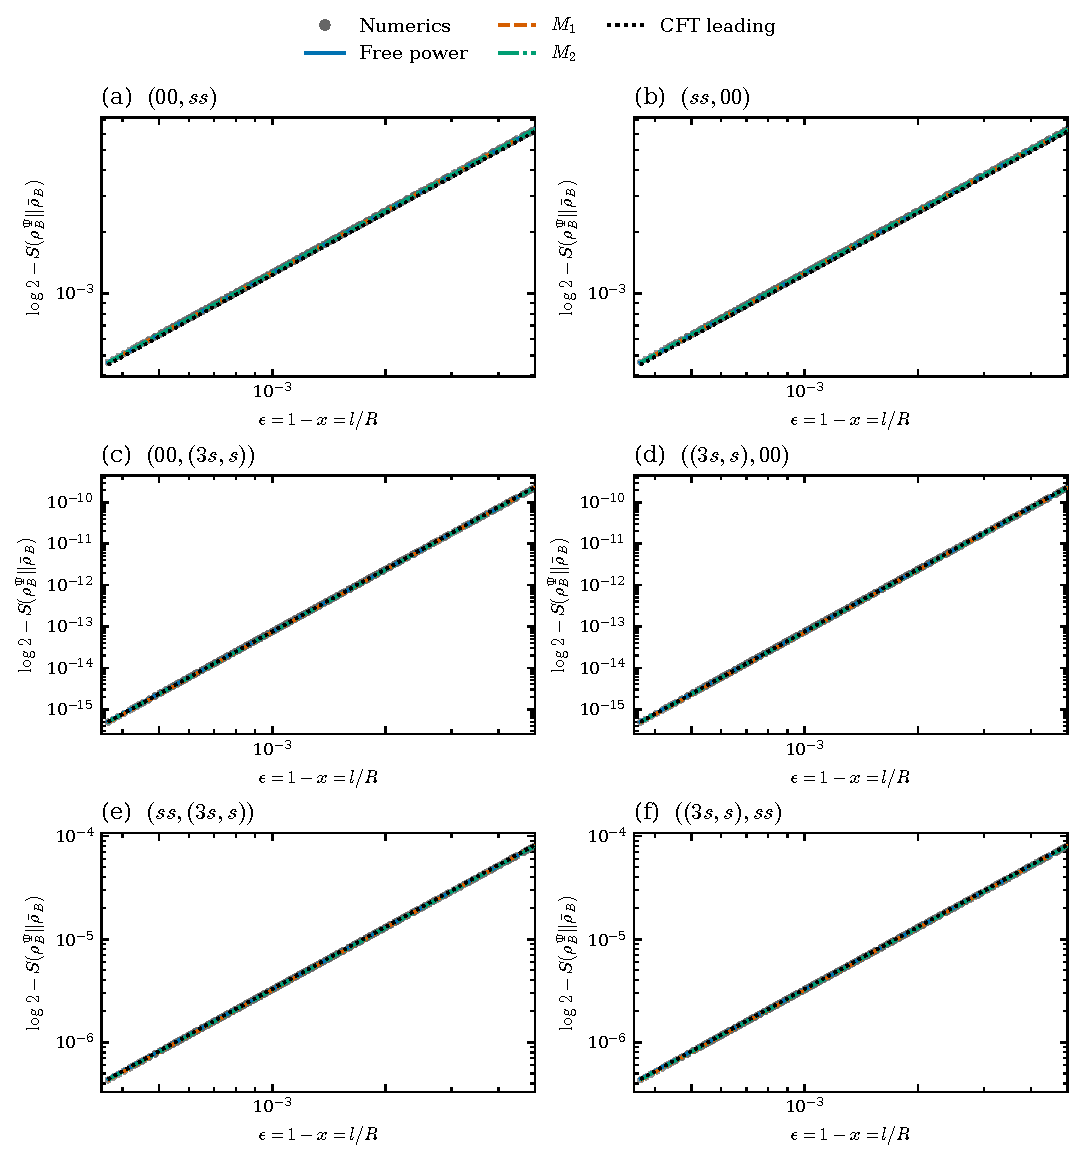
\includegraphics[width=.94\linewidth,height=.74\textheight,keepaspectratio]{figs/boson_large_fit_window_value.pdf}
\caption{Compact-boson large-interval $\delta_{a\mid b}=\log2-D^B_{a\mid b}$ for all six ordered pairs. All 317 displayed geometries per direction lie in the fitting window $0<\ep\leq0.005$, with $\ell=6,\ldots,10$. Both axes are logarithmic. Gray circles denote numerical data, using the same shape and color for every subsystem length. Blue solid, orange dashed, and green dash--dotted curves denote the free fit, $F_1$, and $F_2$; black dotted denotes the parameter-free CFT leading term. All curves are restricted to the fitting window. The horizontal label $y$ denotes the complement fraction $\ep=1-x_B=\ell/N$, while the mixing probability is fixed at $1/2$.}
\label{fig:num-boson-large}
\end{figure}

\begin{figure}[p]\centering
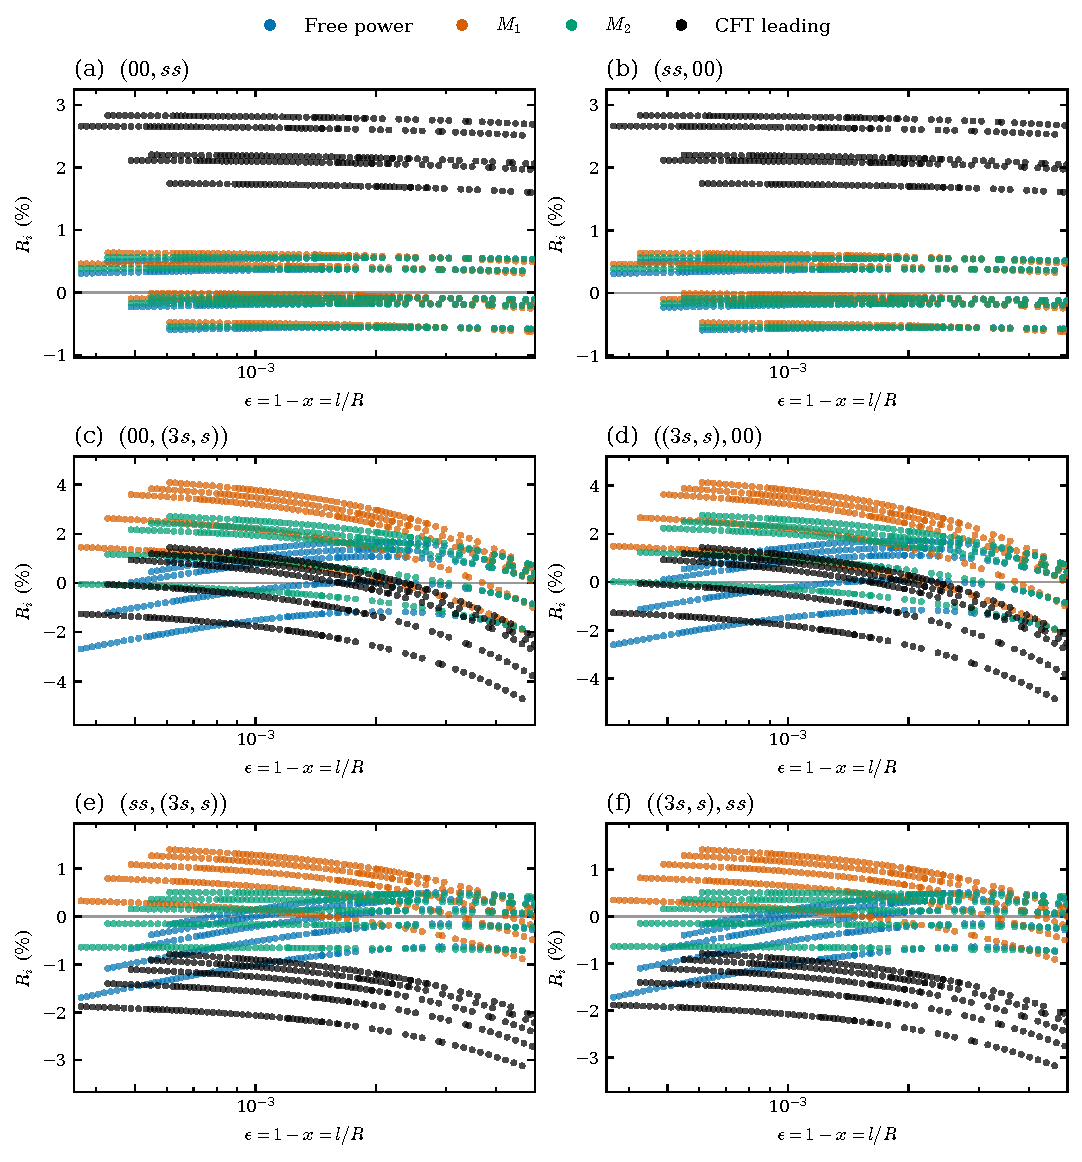
\includegraphics[width=.94\linewidth,height=.74\textheight,keepaspectratio]{figs/boson_large_fit_window_residual.pdf}
\caption{Signed percentage residuals $100[q-M]/q$ for Fig.~\ref{fig:num-boson-large}, with $q=\delta$. The residual ordinate is linear and the fraction axis logarithmic. Only the 317 fitted geometries per direction at $0<\ep\leq0.005$ are shown. All subsystem lengths $\ell=6,\ldots,10$ use circular markers; colors identify models and are identical across lengths. Blue, orange, green, and black denote the free fit, $F_1$, $F_2$, and the parameter-free CFT leading term. The horizontal label $y$ denotes the complement fraction $\ep=1-x_B=\ell/N$, while the mixing probability is fixed at $1/2$.}
\label{fig:num-boson-large-residual}
\end{figure}

\clearpage
